% Each drawn edge represents both directed cube varieties.
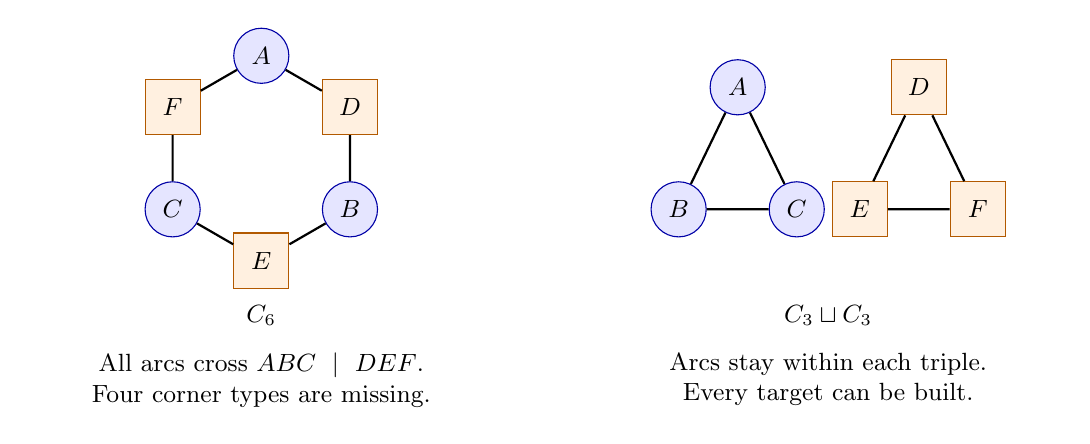
\begin{tikzpicture}[
  every node/.style={font=\small},
  p/.style={circle,draw=blue!65!black,fill=blue!10,minimum size=7mm,inner sep=1pt},
  q/.style={rectangle,draw=orange!70!black,fill=orange!12,minimum size=7mm,inner sep=1pt},
  support/.style={line width=0.8pt},
  explanation/.style={align=center,text width=5.7cm,font=\small}
]
\begin{scope}
  \node[p] (A) at (0,1.3) {$A$};
  \node[q] (D) at (1.126,0.65) {$D$};
  \node[p] (B) at (1.126,-0.65) {$B$};
  \node[q] (E) at (0,-1.3) {$E$};
  \node[p] (C) at (-1.126,-0.65) {$C$};
  \node[q] (F) at (-1.126,0.65) {$F$};
  \draw[support] (A)--(D)--(B)--(E)--(C)--(F)--(A);
  \node at (0,-2.0) {$C_6$};
  \node[explanation,anchor=north] at (0,-2.35)
    {All arcs cross $ABC\mid DEF$.\\
     Four corner types are missing.};
\end{scope}
\begin{scope}[xshift=7.2cm]
  \node[p] (A2) at (-1.15,0.9) {$A$};
  \node[p] (B2) at (-1.9,-0.65) {$B$};
  \node[p] (C2) at (-0.4,-0.65) {$C$};
  \node[q] (D2) at (1.15,0.9) {$D$};
  \node[q] (E2) at (0.4,-0.65) {$E$};
  \node[q] (F2) at (1.9,-0.65) {$F$};
  \draw[support] (A2)--(B2)--(C2)--(A2);
  \draw[support] (D2)--(E2)--(F2)--(D2);
  \node at (0,-2.0) {$C_3\sqcup C_3$};
  \node[explanation,anchor=north] at (0,-2.35)
    {Arcs stay within each triple.\\
     Every target can be built.};
\end{scope}
\end{tikzpicture}
